\newpage
\section{Giới thiệu chung}
\subsection{Giới thiệu chung về OpenMP}
Lập trình đa luồng là một phương pháp lập trình trong đó một chương trình có khả năng thực hiện nhiều công việc đồng thời, mỗi công việc được thực hiện trong một luồng riêng biệt.

OpenMP (Open Multi-Processing) là một giao diện lập trình ứng dụng   hỗ trợ lập trình đa xử lý bộ nhớ dùng chung đa nền tảng trong C , C++ và Fortran.

OpenMP được thiết kế cho các máy đa bộ xử lý/lõi, bộ nhớ dùng chung. Kiến trúc cơ bản có thể là bộ nhớ chia sẻ UMA hoặc NUMA.

\begin{figure}[h] %!nghia
    \centering
    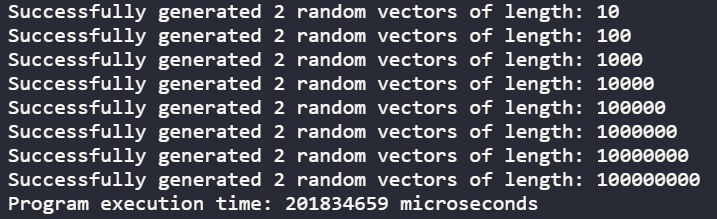
\includegraphics[width=1\textwidth]{pictures/image.png} %!nghia
    \caption{ViDuHinhAnhTheoChieuNgang} %!nghia
    \label{pictures:nghia12} %!nghia
    \end{figure} 


% Fork-Join
% Share memory
 


% #### 2.1 Fork-Join Model
% Mô hình Fork-Join là mô hình cơ bản trong lập trình song song, trong đó một quá trình "cha" tạo ra các quá trình "con" để thực hiện các công việc con. Sau khi các công việc con kết thúc, chúng hợp nhất lại với quá trình cha. OpenMP sử dụng mô hình này để tận dụng hiệu suất từ việc chia nhỏ công việc.


% #### 2.3 Share Memory
% Chia sẻ bộ nhớ là khái niệm trong lập trình song song, trong đó nhiều luồng có thể truy cập cùng một không gian bộ nhớ chung. Trong OpenMP, bộ nhớ chia sẻ giúp các luồng truy cập và cập nhật dữ liệu mà không cần sự sao chép dữ liệu giữa chúng, tăng hiệu suất chương trình.
 
 
 

% OpenMP là một công cụ mạnh mẽ cho lập trình song song, sử dụng mô hình Fork-Join, đa luồng, và chia sẻ bộ nhớ để tối ưu hóa hiệu suất ứng dụng trên các hệ thống có nhiều lõi CPU.  
\subsection{Công thức tính hiệu suất}


Công thức tính hiệu suất:
\begin{equation}
 \text{{Hiệu suất}} = \frac{{\text{{time1}}}}{{\text{{time2}}}} \div \text{{thread}}
\end{equation}


\subsection{Thông tin về máy tính và phần mềm}




 
 
 